\documentclass{article}
\usepackage{amsmath}
\usepackage{graphicx}
\usepackage{float}
\usepackage{hyperref}
\usepackage{fancyvrb}
\usepackage{matlab-prettifier}
\usepackage{subcaption}
\setlength{\parindent}{0pt}
\graphicspath{{../images/}}

\title{CS663: Digital Image Processing - Homework 3}
\author{Harsh $\vert$ Pranav $\vert$ Swayam} 
\date{October 1, 2024}

\begin{document}

\maketitle
\section{Homework 3 - Question 3}

\subsection{Introduction}
In this question, we consider two images: `barbara256.png' and `kodak24.png'. We add zero-mean Gaussian noise with standard deviation $\sigma = 5$ and $\sigma = 10$ to both images. We then apply a mean shift based filter with different parameter configurations and analyze the results.

\subsection{Original Images}
\begin{figure}[H]
    \centering
    \begin{subfigure}[b]{0.45\textwidth}
        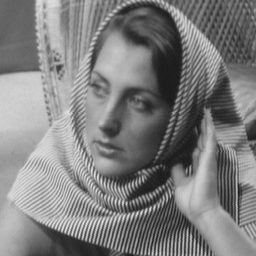
\includegraphics[width=\textwidth]{../images/barbara256.png}
        % \caption{barbara256.png`}
    \end{subfigure}
    \begin{subfigure}[b]{0.45\textwidth}
        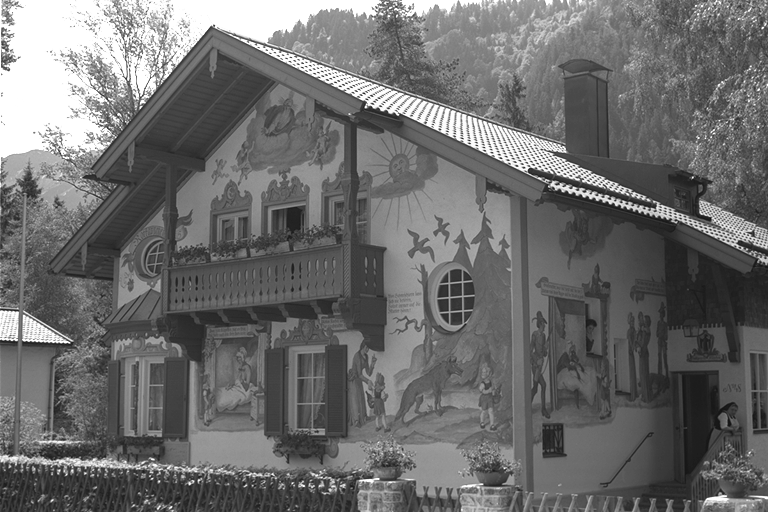
\includegraphics[width=\textwidth]{../images/kodak24.png}
        % \caption{`kodak24.png`}
    \end{subfigure}
    \caption{Original Images}
\end{figure}

\subsection{Noisy Images}
\begin{figure}[H]
    \centering
    \begin{subfigure}[b]{0.45\textwidth}
        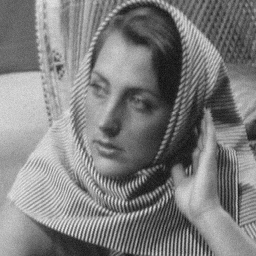
\includegraphics[width=\textwidth]{../images/barbara_5.png}
        % \caption{`barbara256.png`}
    \end{subfigure}
    \begin{subfigure}[b]{0.45\textwidth}
        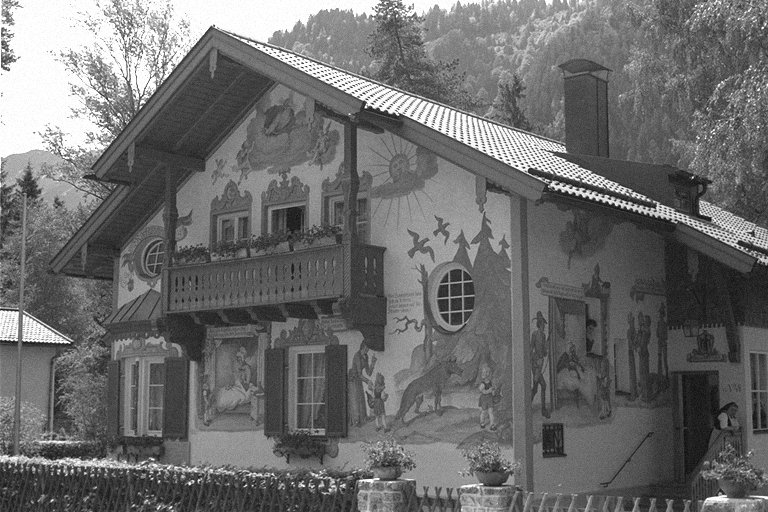
\includegraphics[width=\textwidth]{../images/kodak_5.png}
        % \caption{`kodak24.png`}
    \end{subfigure}
    \caption{Images corrupted with zero-mean Gaussian noise ($\sigma = 5$).}
\end{figure}

\begin{figure}[H]
    \centering
    \begin{subfigure}[b]{0.45\textwidth}
        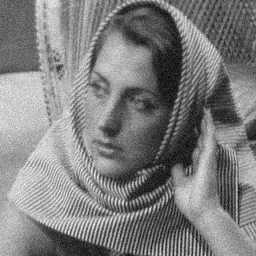
\includegraphics[width=\textwidth]{../images/barbara_10.png}
        % \caption{`barbara256.png`}
    \end{subfigure}
    \begin{subfigure}[b]{0.45\textwidth}
        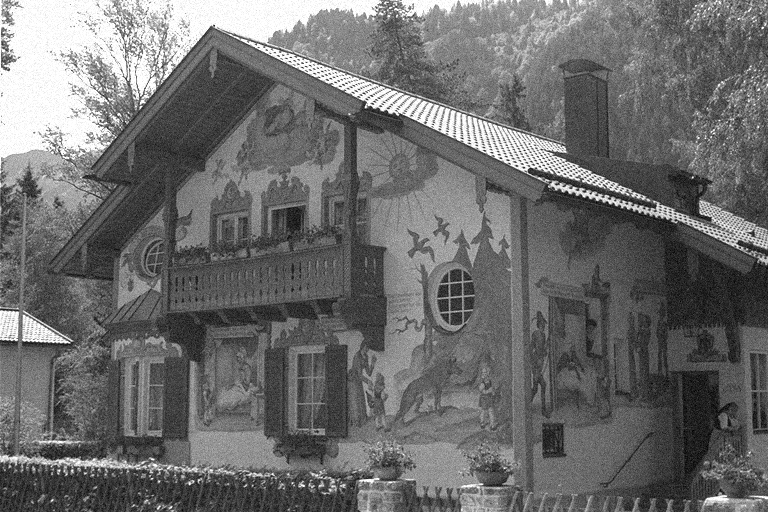
\includegraphics[width=\textwidth]{../images/kodak_10.png}
        % \caption{`kodak24.png`}
    \end{subfigure}
    \caption{Images corrupted with zero-mean Gaussian noise ($\sigma = 10$).}
\end{figure}

\subsection{Mean Shift Filter Results}
\subsubsection{Parameter Configuration: $\sigma_s = 2$, $\sigma_r = 2$}
\begin{figure}[H]
    \centering
    \begin{subfigure}[b]{0.45\textwidth}
        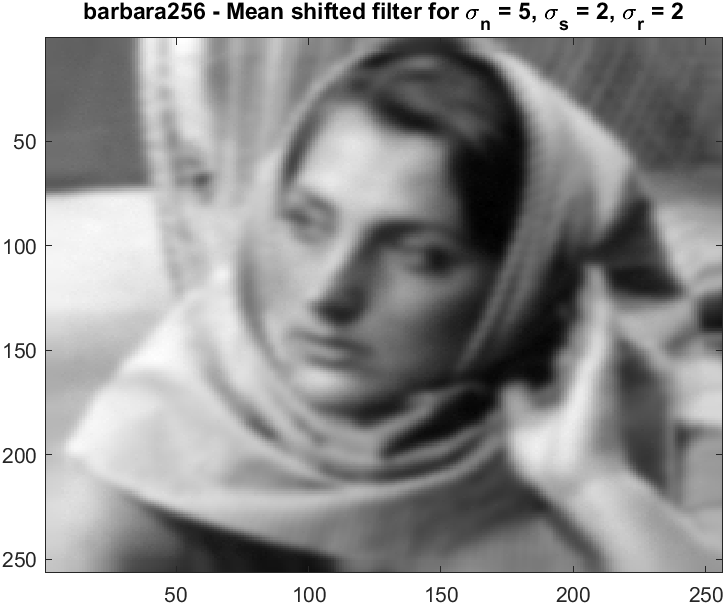
\includegraphics[width=\textwidth]{../images/barbara_5_2_2.png}
        % \caption{`barbara256.png`}
    \end{subfigure}
    \begin{subfigure}[b]{0.45\textwidth}
        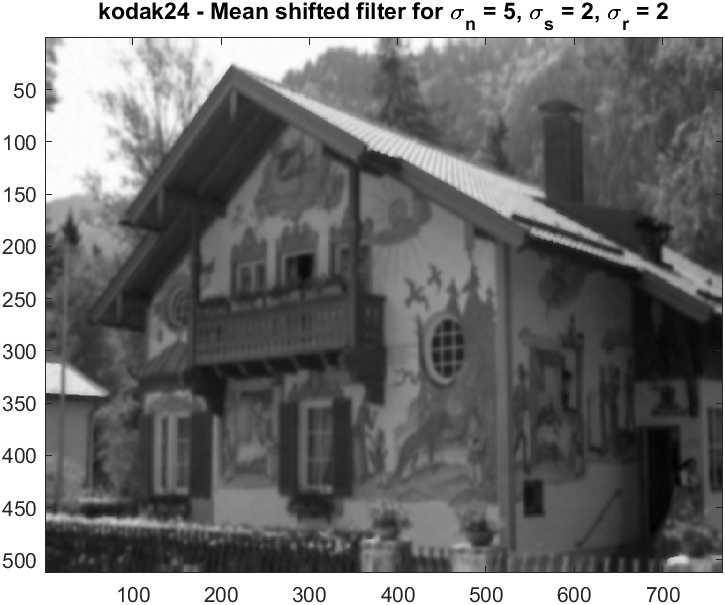
\includegraphics[width=\textwidth]{../images/kodak_5_2_2.png}
        % \caption{`kodak24.png`}
    \end{subfigure}
    \caption{Mean shift filter results ($\sigma = 5$, $\sigma_s = 2$, $\sigma_r = 2$).}
\end{figure}

\begin{figure}[H]
    \centering
    \begin{subfigure}[b]{0.45\textwidth}
        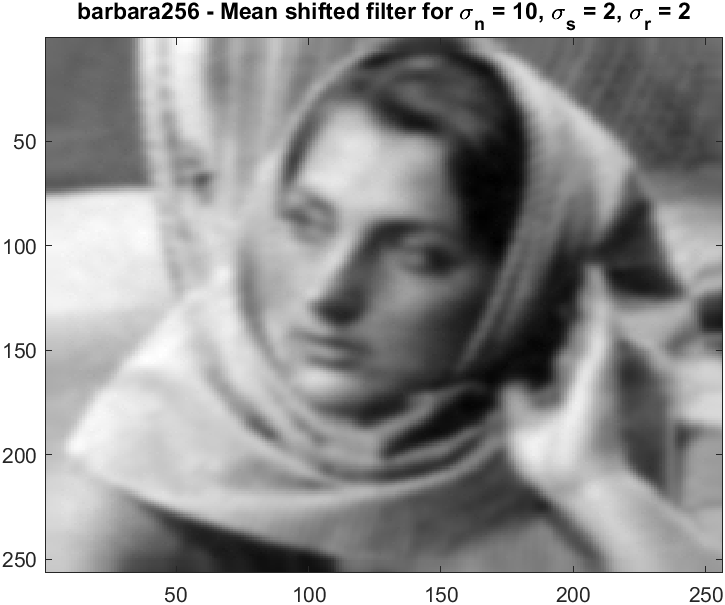
\includegraphics[width=\textwidth]{../images/barbara_10_2_2.png}
        % \caption{`barbara256.png`}
    \end{subfigure}
    \begin{subfigure}[b]{0.45\textwidth}
        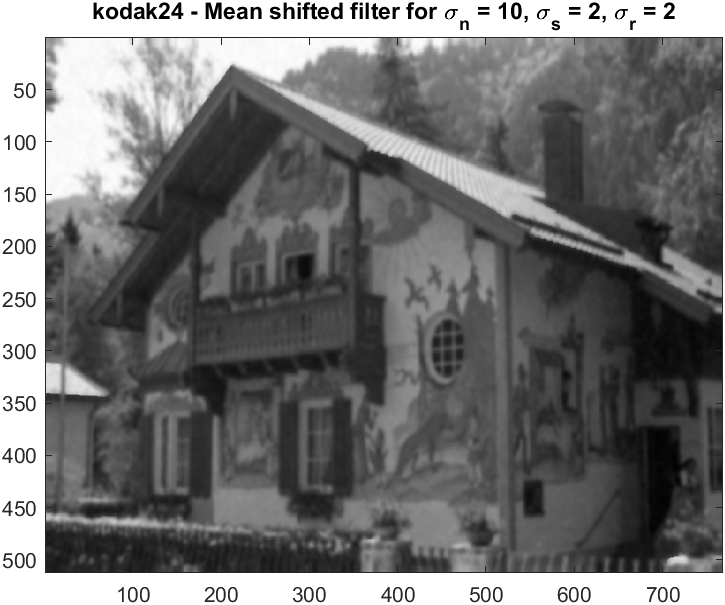
\includegraphics[width=\textwidth]{../images/kodak_10_2_2.png}
        % \caption{`kodak24.png`}
    \end{subfigure}
    \caption{Mean shift filter results ($\sigma = 10$, $\sigma_s = 2$, $\sigma_r = 2$).}
\end{figure}

\subsubsection{Parameter Configuration: $\sigma_s = 15$, $\sigma_r = 3$}

The attainment of convergence takes a longer time for this configuration due to a higher spatial bandwidth leading to very slow convergence and hence the results were not attained in the observed time ($\sim$ 15 minutes). Reasons for this are explained in the observations section in detail.

\subsubsection{Parameter Configuration: $\sigma_s = 3$, $\sigma_r = 15$}
\begin{figure}[H]
    \centering
    \begin{subfigure}[b]{0.45\textwidth}
        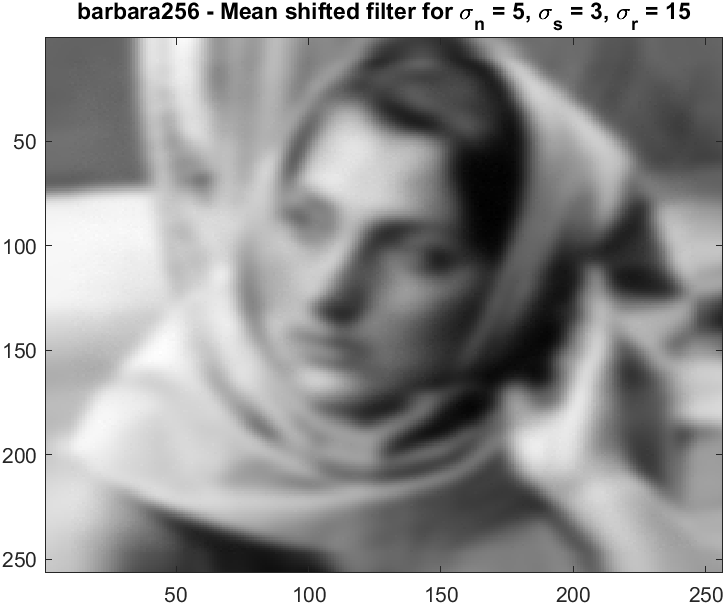
\includegraphics[width=\textwidth]{../images/barbara_5_3_15.png}
        % \caption{`barbara256.png`}
    \end{subfigure}
    \begin{subfigure}[b]{0.45\textwidth}
        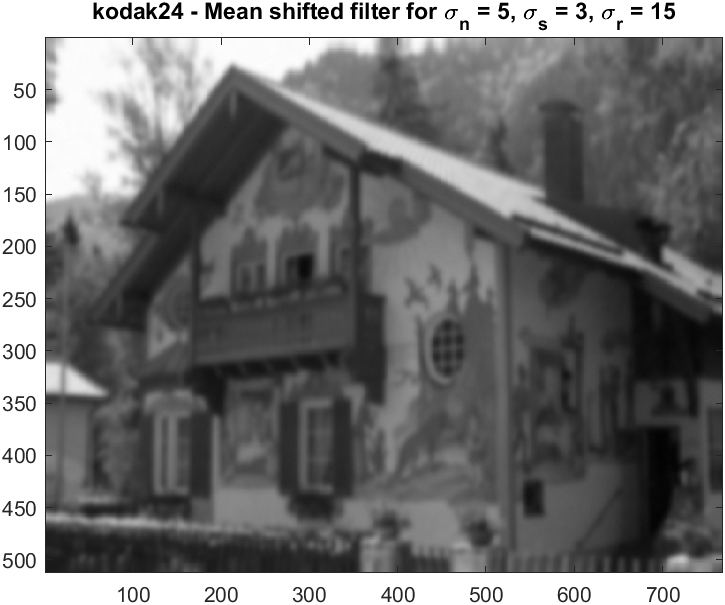
\includegraphics[width=\textwidth]{../images/kodak_5_3_15.png}
        % \caption{`kodak24.png`}
    \end{subfigure}
    \caption{Mean shift filter results ($\sigma = 5$, $\sigma_s = 3$, $\sigma_r = 15$).}
\end{figure}

\begin{figure}[H]
    \centering
    \begin{subfigure}[b]{0.45\textwidth}
        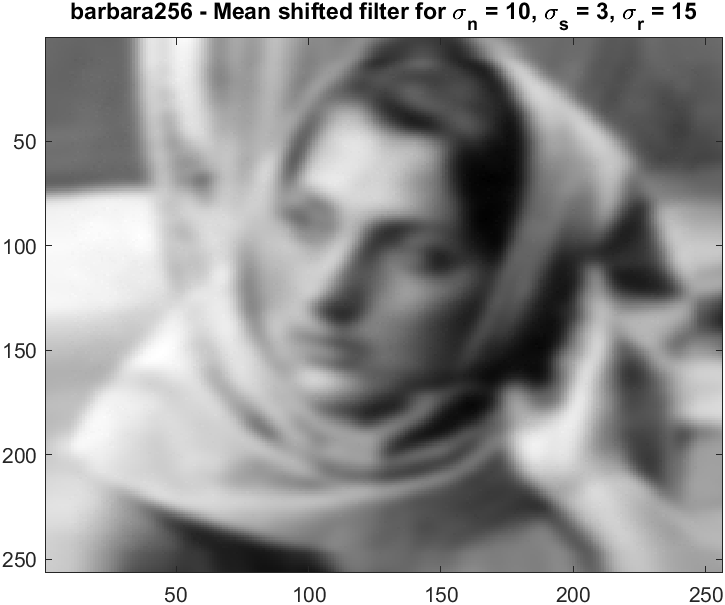
\includegraphics[width=\textwidth]{../images/barbara_10_3_15.png}
        % \caption{`barbara256.png`}
    \end{subfigure}
    \begin{subfigure}[b]{0.45\textwidth}
        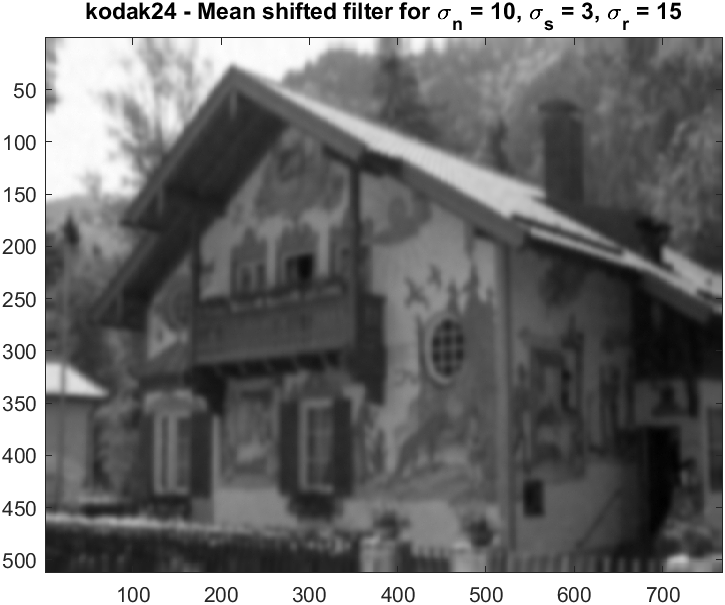
\includegraphics[width=\textwidth]{../images/kodak_10_3_15.png}
        % \caption{`kodak24.png`}
    \end{subfigure}
    \caption{Mean shift filter results ($\sigma = 10$, $\sigma_s = 3$, $\sigma_r = 15$).}
\end{figure}

\subsection{Observations}
\begin{itemize}
    \item For $\sigma_s$:
    \begin{itemize}
        \item As it increases, a larger and larger neighborhood of values around $p = (x, y)$ will contribute to the averaging (more noise reduction but possible contribution from dissimilar regions)
        \item For higher values of $\sigma_s$ (the spatial bandwidth), convergence tends to be slow or may not be reached because the algorithm searches over a much larger neighborhood in the spatial domain. This means:
        \begin{itemize}
            \item A larger $\sigma_s$ causes the algorithm to consider a broader area around each pixel when computing the weighted mean shift, resulting in smaller shifts per iteration since the influence of far-away points dilutes the update.
            \item As the spatial weights (Gaussian kernel) are spread over a larger area, the gradient of the weight function becomes flatter, making it harder for the algorithm to push the feature vector towards a stable mode quickly.
        \end{itemize}
    \end{itemize}
    \item For $\sigma_r$:
    \begin{itemize}
        \item For moderate values, only intensities close to $I(p)$ will affect the averaging
        \item Features or edges with intensity difference less than $\sigma_r$ will be blurred, others will be preserved
        \item A behavior similar to $\sigma_s$ isn't seen with $\sigma_r$ (the range bandwidth) because $\sigma_r$ controls the sensitivity to intensity differences (or range differences), not spatial differences. This results in convergence being reached more easily with higher values of $\sigma_r$ as seen in the third configuration.
    \end{itemize}
\end{itemize}

Thus, for higher value of $\sigma_s$, the edges are not very well preserved and for very high values convergence is not attained in a feasible duration. For higher value of $\sigma_r$, more averaging occurs compared to smaller values.

As $\sigma_n$ increases, that is, the noise added increases and higher mean shift filtering is required to smoothen the image (like in the case of $\sigma_s = 3, \sigma_r = 15$).


\end{document}